برای این پلتفرم، سیستم را به دامنه‌های مجزا با مالکیت داده اختصاصی (\lr{Database-per-Service}) تقسیم می‌کنیم:
\begin{itemize}
    \item {سرویس احراز هویت و کاربران (\lr{Auth \& User Service}):} مدیریت ثبت‌نام، پروفایل دانشجویان/مدرسان و نقش‌ها.
    \item {سرویس کاتالوگ دوره‌ها (\lr{Course Catalog Service}):} مشاهده دوره‌ها، جستجو و بارگذاری محتوا (ویدئوها و متون) توسط مدرسان.
    \item {سرویس سفارش و پرداخت (\lr{Order \& Payment Service}):} مدیریت سبد خرید، صدور فاکتور و اتصال به درگاه پرداخت.
    \item {سرویس تعاملی و تمرین‌ها (\lr{Progress \& Assignment Service}):} ثبت وضعیت پیشرفت دانشجو، ارسال تمرین‌ها و فرآیند تصحیح.
    \item {سرویس گواهی‌نامه (\lr{Certificate Service}):} صدور و اعتبارسنجی گواهی پایان دوره به صورت خودکار.
    \item {سرویس پیشنهادات و رتبه‌بندی (\lr{Recommendation \& Review Service}):} ثبت امتیازها و سیستم پیشنهاد دوره بر اساس رفتارهای قبلی کاربر.
    \item {سرویس اعلان‌ها (\lr{Notification Service}):} ارسال ایمیل، پیامک و اعلان‌های درون‌برنامه‌ای در زمان کمپین‌ها یا انتشار دوره جدید.
\end{itemize}

جهت حفظ پایداری و کارایی سیستم در زمان اوج ترافیک، الگوهای ارتباطی زیر پیاده‌سازی می‌شوند:
\begin{enumerate}
    \item {ارتباط همگام (\lr{Synchronous - HTTP/gRPC}):}
    \begin{itemize}
        \item {کاربرد:} در لایه \lr{API Gateway} برای هدایت درخواست‌های مستقیم کاربر و همچنین در مواقعی که نیاز به پاسخ آنی است؛ مانند تایید نهایی تراکنش توسط \lr{Payment Service} که \lr{Order Service} باید فوراً از آن مطلع شود.
    \end{itemize}
    \item {ارتباط ناهمگام (\lr{Asynchronous - Event-Driven via Message Broker}):}
    \begin{itemize}
        \item {خرید موفق:} پس از پرداخت، \lr{Payment Service} رویداد \lr{OrderPaid} را منتشر می‌کند. سرویس‌های تعاملی (برای باز شدن دسترسی دوره)، گواهی‌نامه (برای بررسی وضعیت نهایی بعداً) و اعلان‌ها این رویداد را مصرف می‌کنند.
        \item {انتشار دوره جدید یا کمپین:} سرویس کاتالوگ رویداد \lr{CoursePublished} را منتشر کرده و \lr{Notification Service} به صورت ناهمگام شروع به ارسال ایمیل‌های گروهی بدون درگیر کردن منابع اصلی وب‌سایت می‌کند.
    \end{itemize}
\end{enumerate}

با توجه به مجزا بودن دیتابیس‌ها، امکان استفاده از \lr{ACID} سنتی وجود ندارد. برای فرآیندهای چندمرحله‌ای مثل «خرید دوره $\leftarrow$ کسر موجودی/تایید درگاه $\leftarrow$ فعال‌سازی دسترسی دوره»، از {الگوی ساگا (\lr{Saga Pattern})} مبتنی بر ارکستراسیون استفاده می‌شود:
\begin{itemize}
    \item {تراکنش‌های جبرانی:} اگر در مرحله آخر (مثلاً فعال‌سازی دوره) خطایی رخ دهد، رویداد جبرانی (\lr{Rollback Event}) صادر می‌شود تا تراکنش مالی در سرویس پرداخت برگشت داده شود (\lr{Refund}) و سیستم به وضعیت پایدار قبلی برسد.
\end{itemize}

با توجه به اینکه در زمان کمپین‌ها تعداد کاربران به طور ناگهانی افزایش می‌یابد، تمهیدات زیر الزامی است:
\begin{itemize}
    \item {\lr{Auto-scaling} در سطح کانتینرها:} استفاده از کلاستر \lr{Kubernetes} و تنظیم \lr{HPA} بر اساس میزان مصرف \lr{CPU} و نرخ درخواست‌ها، تا سرویس‌های پرمصرف مثل کاتالوگ و احراز هویت به سرعت تکثیر شوند.
    \item {لایه کشینگ توزیع‌شده:} استفاده از \lr{Redis} برای کش کردن اطلاعات سنگین و پربازدید (مانند ساختار دوره‌ها و ویدئوها) تا فشار روی پایگاه داده‌های اصلی کاهش یابد.
    \item {کنترل نرخ درخواست (\lr{Rate Limiting}):} پیاده‌سازی الگوریتم‌های \lr{Rate Limiting} در سطح \lr{API Gateway} برای جلوگیری از حملات \lr{DDoS} و مسدود کردن درخواست‌های مخرب یا اسپم در زمان کمپین‌ها.
    \item {ضربه‌گیری با \lr{Message Broker}:} هدایت حجم عظیمی از کارهای غیرضروری (مثل ثبت لاگ‌های پیشرفت ویدئو یا صف‌های ارسال اعلان) به ابزارهایی مانند \lr{Kafka} یا \lr{RabbitMQ} جهت تعدیل بار.
\end{itemize}


$\\$

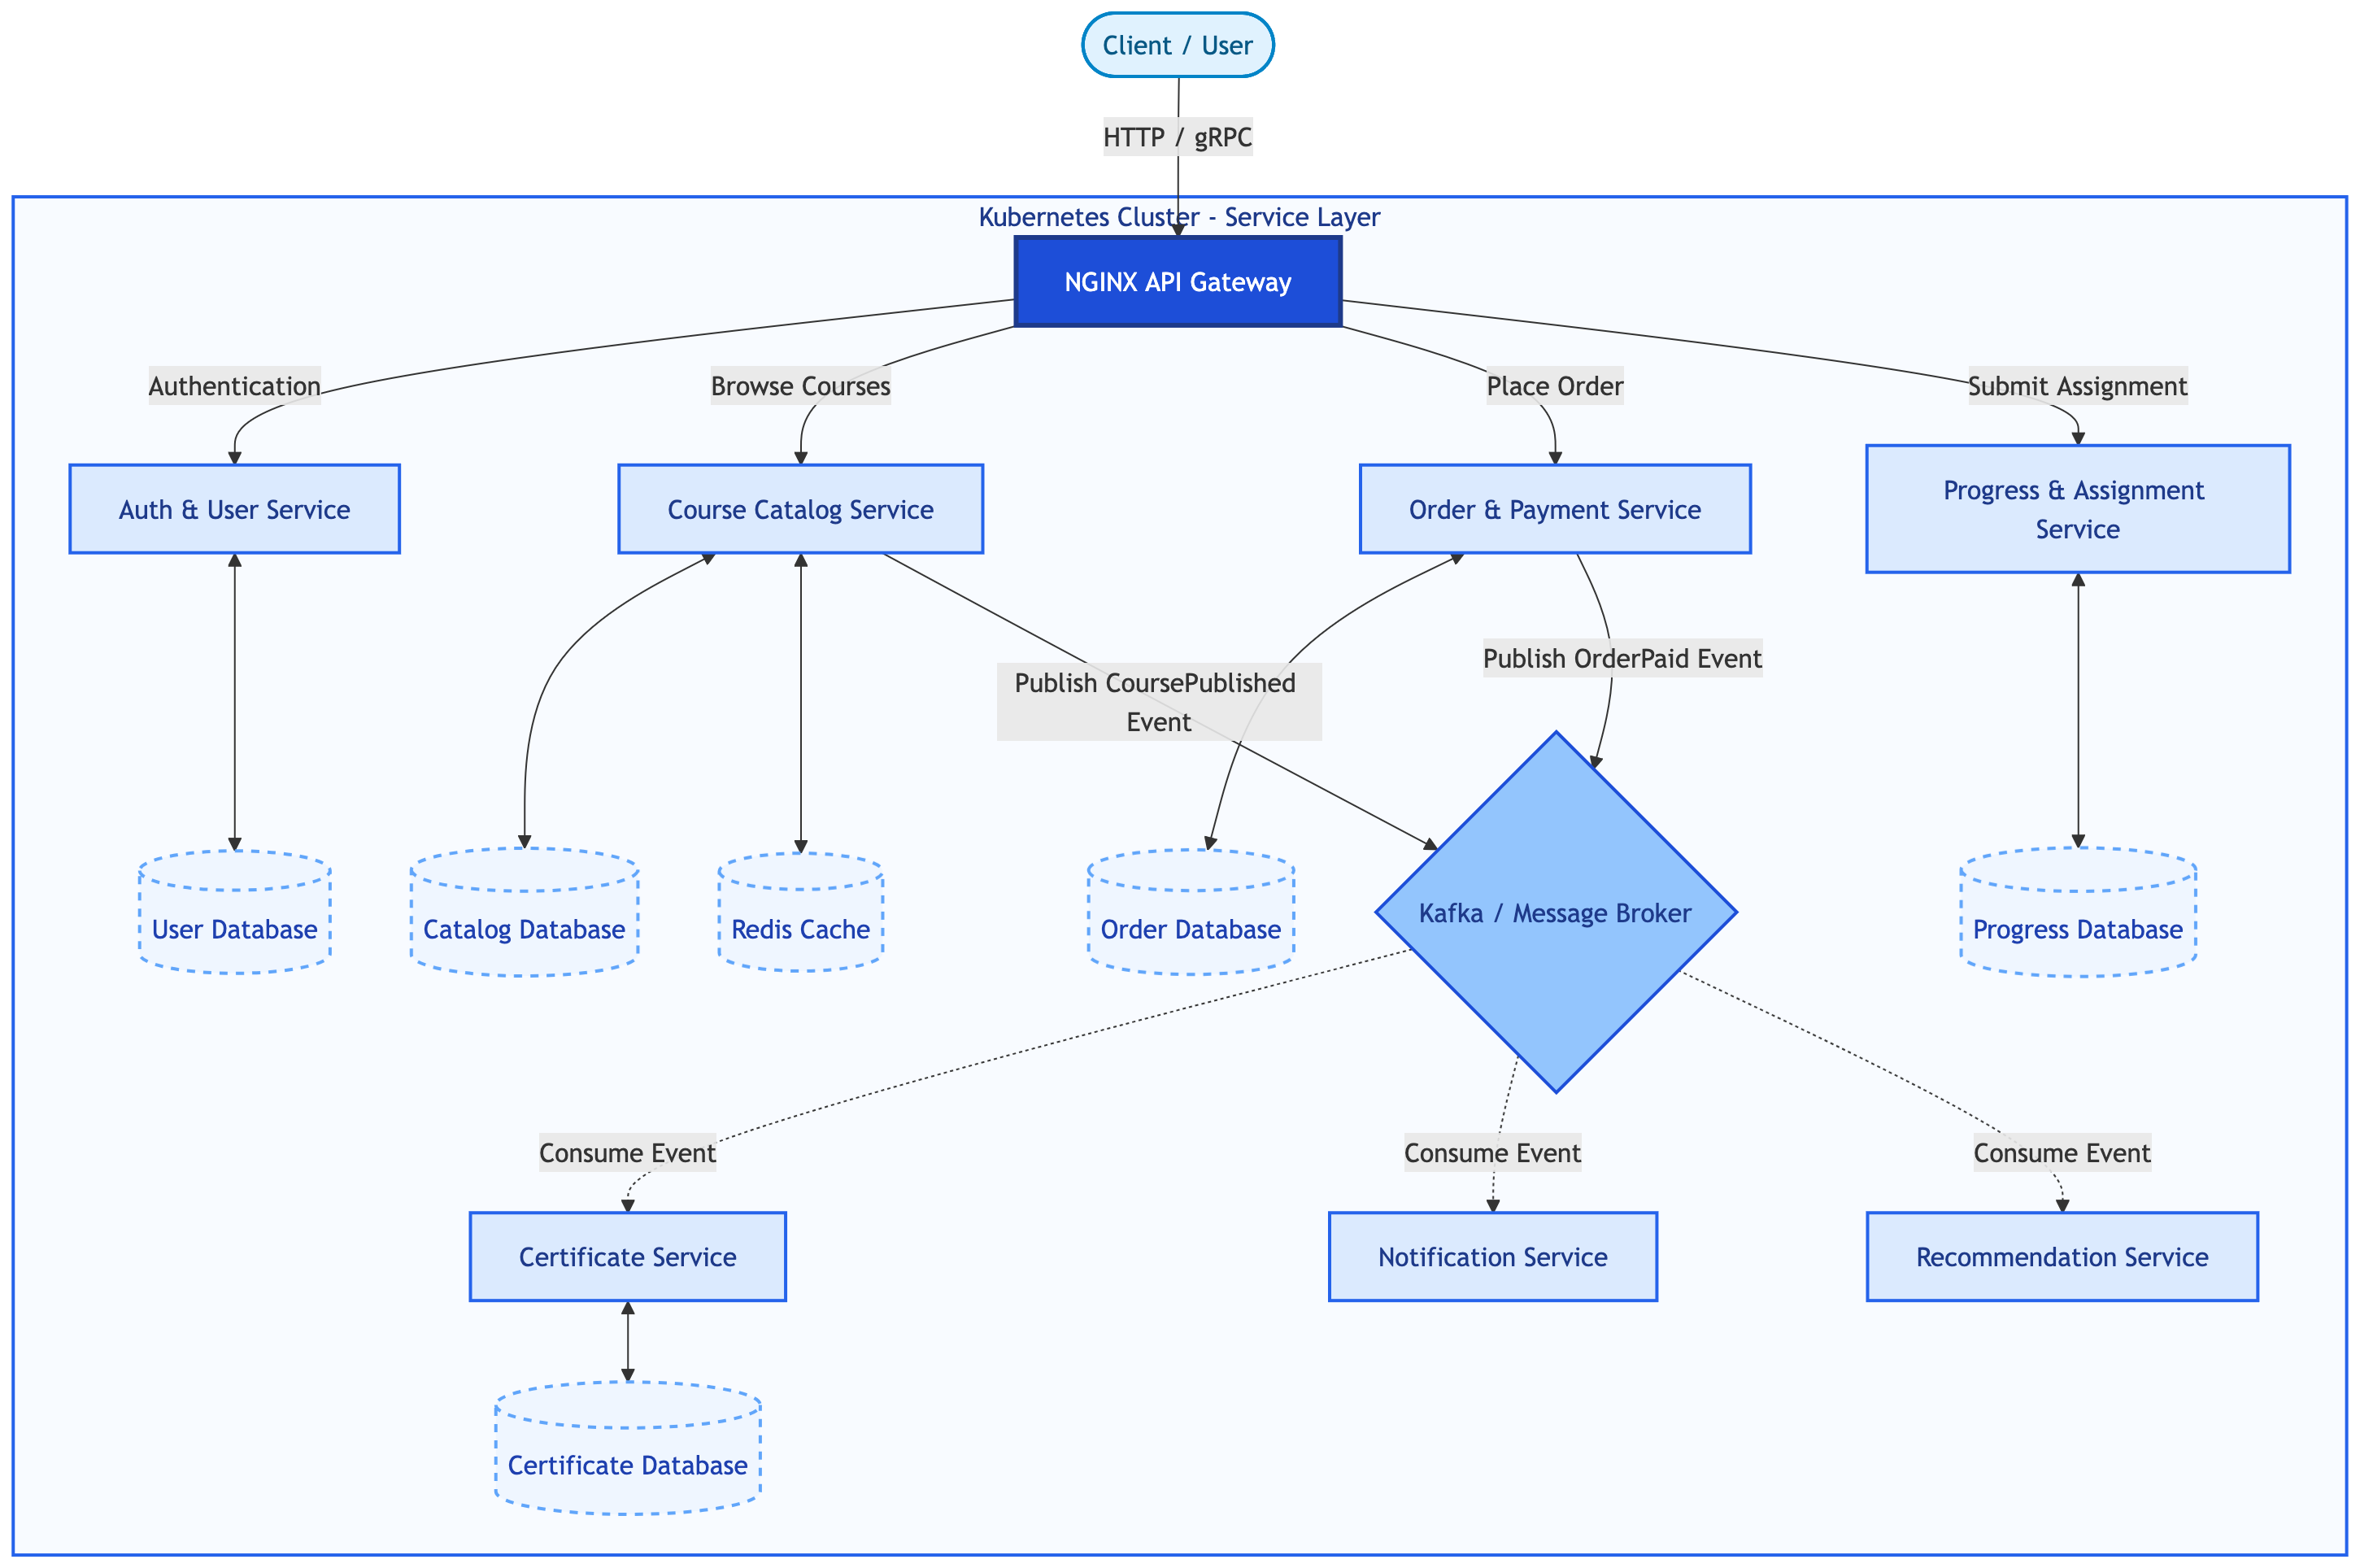
\includegraphics[width=1\textwidth]{figs/2.png}